\documentclass[12pt]{beamer}
\usepackage{cmap}
\usepackage[T2A]{fontenc}
\usepackage[utf8]{inputenc}
\usepackage{ifluatex}
\usefonttheme[onlymath]{serif}
\usepackage{svg}
\usepackage{enumerate}
\usepackage{hyperref}
\usepackage{mathtools}

\definecolor{beamer@darkgreen}{rgb}{0,0.6,0}
\setbeamercolor{normal text}{fg=black,bg=white}
\setbeamercolor{title}{fg=black,bg=beamer@darkgreen}
\setbeamercolor{frametitle}{fg=black,bg=beamer@darkgreen}
\setbeamercolor{background canvas}{parent=normal text}
\setbeamertemplate{footline}[frame number]
\usepackage[english,russian]{babel}
\usepackage{graphicx}
\usepackage{listings}

\author{Катя Тузова}
\title{Машинное обучение}
\subtitle{Лекция 3. Методы кластеризации}
\date{}

\begin{document}
\frame{\titlepage}


\begin{frame}\frametitle{Разбор летучки}
\end{frame}

\begin{frame}\frametitle{Постановка задачи кластеризации}
Кластеризация -- задача разделения объектов одной природы на несколько групп так, чтобы объекты в одной группе обладали одним и тем же свойством.\\
\vspace{5mm}
Кластеризация -- это обучение без учителя.
\end{frame}

\begin{frame}\frametitle{Постановка задачи кластеризации}
$X$ -- пространство объектов\\
$\rho: X \times X \rightarrow [0, \infty)$ -- функция расстояния между объектами\\
\vspace{5mm}
Найти:\\
$Y$ -- множество кластеров \\
$a: X \rightarrow Y$ -- алгоритм кластеризации
\vspace{5mm}

\end{frame}

\begin{frame}\frametitle{Степени свободы в постановке задачи}
	\begin{itemize}
		\item[--] Критерий качества кластеризации
		\item[--] Число кластеров неизвестно заранее
		\item[--] Результат кластеризации существенно зависит от метрики
	\end{itemize}
\end{frame}

\begin{frame}\frametitle{Цели кластеризации}
	\begin{itemize}
		\item[--] Сократить объём хранимых данных
		\item[--] Выделить нетипичные объекты
		\item[--] Упростить дальнейшую обработку данных
		\item[--] Построить иерархию множества объектов				
	\end{itemize}
\end{frame}

\begin{frame}\frametitle{Оценка качества кластеризации}
Есть несколько разбиений на кластеры. Как их сравнить?
\end{frame}

\begin{frame}\frametitle{Оценка качества кластеризации}
\begin{itemize}
\item[--] Минимизировать среднее внутрикластерное расстояние\\
\vspace{5mm}
${\frac{\sum\limits_{a(x_i) = a(x_j)} \rho(x_i, x_j)}{\sum\limits_{a(x_i) = a(x_j)} 1} \rightarrow \min}$
\item[--] Максимизировать среднее межкластерное расстояние\\
\vspace{5mm}
${\frac{\sum\limits_{a(x_i) \neq a(x_j)} \rho(x_i, x_j)}{\sum\limits_{a(x_i) \neq a(x_j)} 1} \rightarrow \max}$
\end{itemize}
\end{frame}

\begin{frame}\frametitle{Методы кластеризации}
\begin{itemize}
\item[--] Иерархические
\item[--] Графовые 
\item[--] Статистические 
\end{itemize}
\end{frame}

\begin{frame}\frametitle{Графовые алгоритмы}
Какие есть две очевидные идеи?
\end{frame}

\begin{frame}\frametitle{Графовые алгоритмы}
Очевидные:\\
\begin{itemize}
\item[--] Выделение связных компонент
\item[--] Минимальное покрывающее дерево
\end{itemize}
\end{frame}

\begin{frame}\frametitle{Выделение связных компонент}
\begin{itemize}
\item[--] Рисуем полный граф с весами, равными расстоянию между объектами
\item[--] Выбираем лимит расстояния $r$ и выкидываем все ребра длиннее $r$
\item[--] Компоненты связности полученного графа -- наши кластеры
\end{itemize}
\end{frame}

\begin{frame}\frametitle{Выделение связных компонент}
Как искать компоненты связности?
\end{frame}

\begin{frame}\frametitle{Минимальное покрывающее дерево}
Минимальное остовное дерево -- дерево, содержащее все вершины графа и имеющее минимальный суммарный вес ребер.\\
\vspace{5mm}
Как найти?
\end{frame}

\begin{frame}\frametitle{Минимальное покрывающее дерево}
Как использовать минимальное остовное дерево для разбиения на кластеры?
\end{frame}
\begin{frame}\frametitle{Минимальное покрывающее дерево}
Строим минимальное остовное дерево, а потом выкидываем из него ребра максимального веса.\\
\vspace{5mm}
Сколько ребер выбросим -- столько кластеров получим.
\end{frame}

\begin{frame}\frametitle{Статистические алгоритмы}
\end{frame}

\begin{frame}\frametitle{Алгоритм FOREL}
Input: X, R\\
${U = X, C = 0}$\\\vspace{2mm}
while ${U \neq 0}$:\\
\hspace{5mm} выбрать случайную точку $x_0$\\
\vspace{2mm}
\hspace{5mm} Повторять пока $x_0$ не стабилизируется:\\
\vspace{2mm}
\hspace{10mm} ${c = \left\{ x \in X \vert \rho(x, x_0) < R \right\}}$ \\
\vspace{2mm}
\hspace{10mm} $x_0 = \frac{1}{\vert c \vert} \sum\limits_{x \in c} x$\\
\vspace{2mm}
\hspace{5mm} ${U = U \setminus c}$, ${C = C \cup \left\{ c \right\}}$
\end{frame}

\begin{frame}\frametitle{Алгоритм FOREL}

\begin{itemize}
\item+] Наглядность
\item[+] Сходимость
\item[--] Зависимость от выбора $x_0$
\item[--] Плохо работает, если изначальная выборка плохо делится на кластеры
\end{itemize}

\end{frame}

\begin{frame}\frametitle{Метод $k$-средних}
Идея:\\  минимизировать меру ошибки\\
\vspace{5mm}${E(X, C) = \sum\limits_{i = 1}^n \Vert x_i -\mu_i \Vert^2}$\\
\vspace{5mm}
$\mu_i$ -- ближайший к $x_i$ центр кластера
\end{frame}

\begin{frame}\frametitle{Метод $k$-средних}
Инициализировать центры $k$ кластеров \\
\vspace{2mm}
Пока $c_i$ не перестанет меняться:\\
\hspace{5mm} $c_i = \arg\min\limits_{c \in C} \rho(x_i, \mu_c)$ \hspace{5mm} $i = 1,\dots, l$\\
\vspace{2mm}\hspace{5mm} ${\mu_c = \frac{\sum\limits_{c_i = c} f_j(x_i)}{\sum\limits_{c_i = c} 1} }$ \hspace{10mm} $j = 1,\dots, n$, $c \in C$\\
\vspace{2mm}
$\mu_c$ -- новое положение центров кластеров\\
$c_i$ -- принадлежность $x_i$ к кластеру\\
$\rho(x_i, \mu_c)$ -- расстояние от $x_i$ до центра кластера $\mu_c$
\end{frame}

\begin{frame}\frametitle{Метод $k$-средних}
\begin{figure}[htbp]
  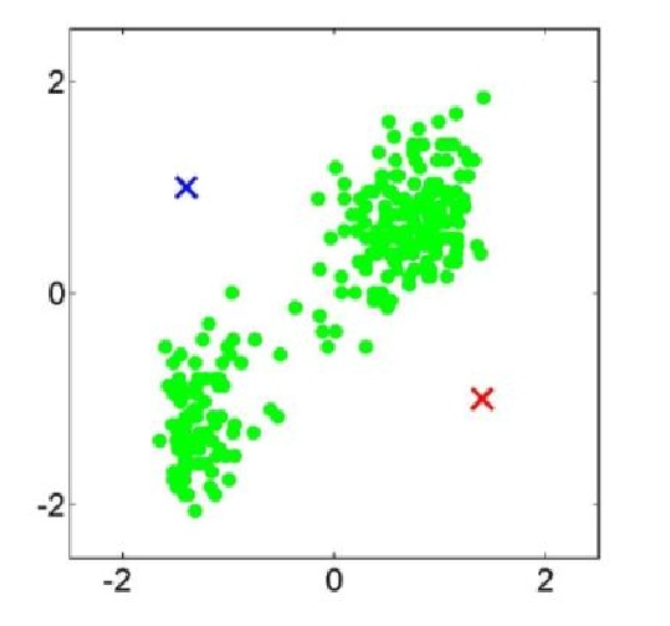
\includegraphics[height=190pt, keepaspectratio = true]{images/k-means-1}   
\end{figure}
\end{frame}

\begin{frame}\frametitle{Метод $k$-средних}
\begin{figure}[htbp]
  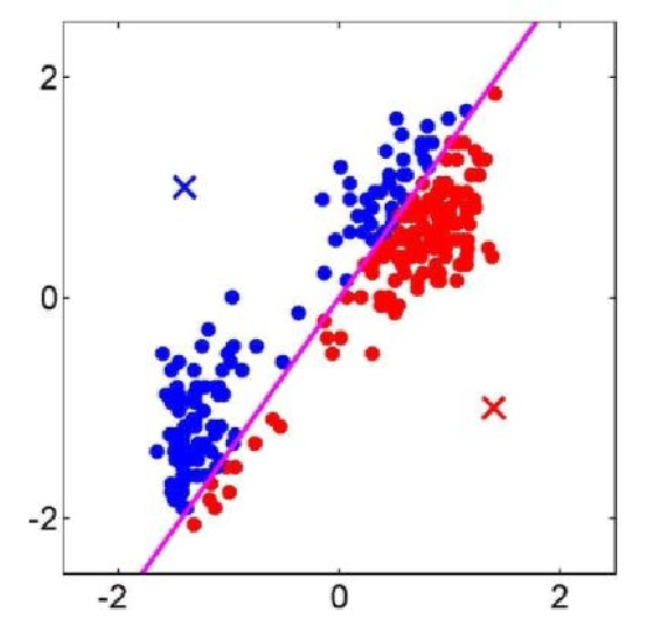
\includegraphics[height=190pt, keepaspectratio = true]{images/k-means-2}   
\end{figure}
\end{frame}

\begin{frame}\frametitle{Метод $k$-средних}
\begin{figure}[htbp]
  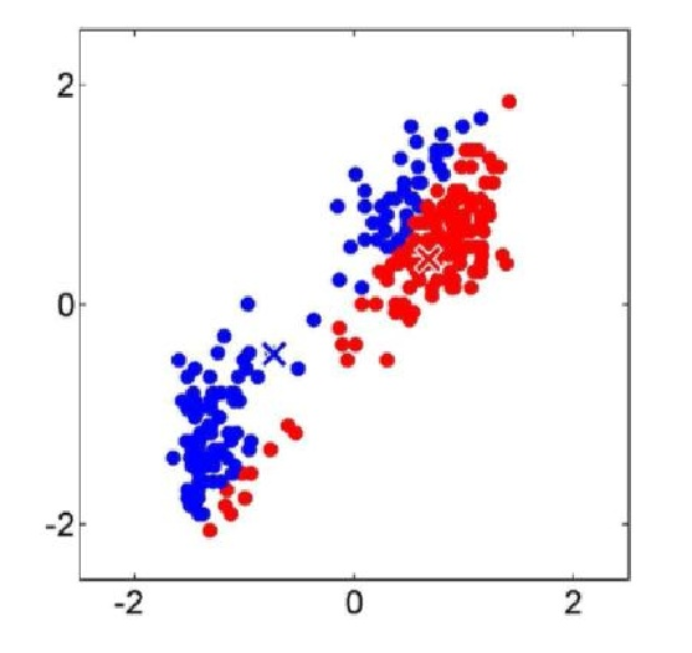
\includegraphics[height=190pt, keepaspectratio = true]{images/k-means-3}   
\end{figure}
\end{frame}

\begin{frame}\frametitle{Метод $k$-средних}
\begin{figure}[htbp]
  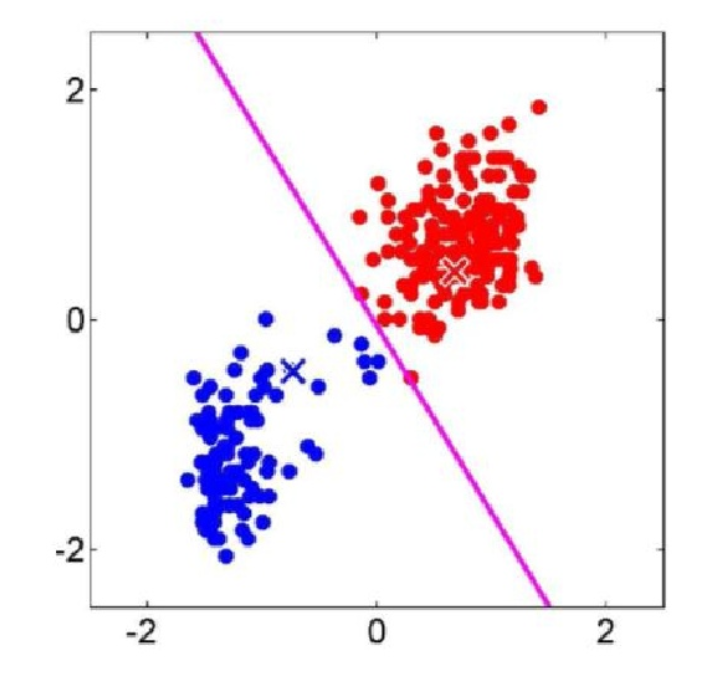
\includegraphics[height=190pt, keepaspectratio = true]{images/k-means-4}   
\end{figure}
\end{frame}

\begin{frame}\frametitle{Метод $k$-средних}
\begin{figure}[htbp]
  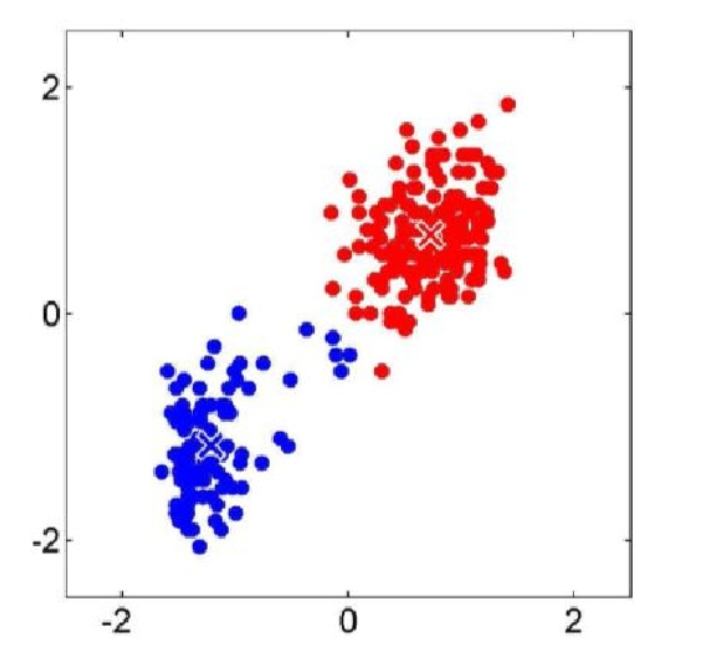
\includegraphics[height=190pt, keepaspectratio = true]{images/k-means-5}   
\end{figure}
\end{frame}

\begin{frame}\frametitle{Особенности метода $k$-средних}
\begin{itemize}
\item[--] Чувствительность к начальному выбору $\mu_c$
\item[--] Необходимость задавать $k$
\end{itemize}
Как устранить эти недостатки?
\end{frame}

\begin{frame}\frametitle{Чувствительность к начальному выбору $\mu_c$}
\begin{figure}[htbp]
  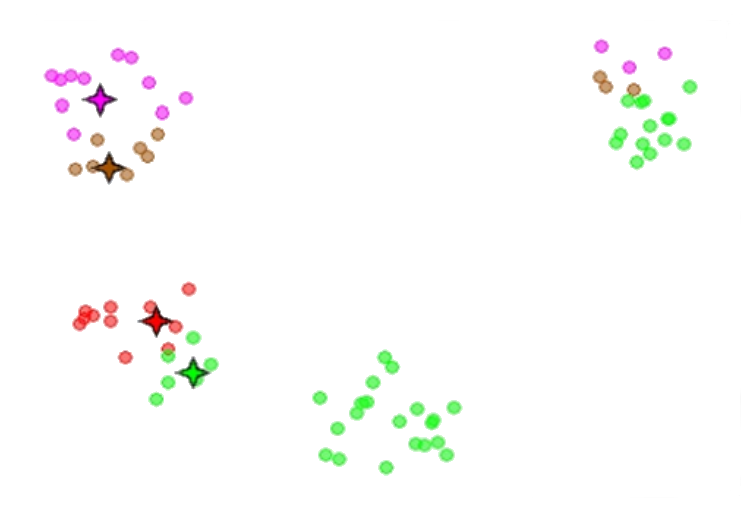
\includegraphics[height=180pt, keepaspectratio = true]{images/local_min2}  
\end{figure}
\end{frame}

\begin{frame}\frametitle{Чувствительность к начальному выбору $\mu_c$}
\begin{figure}[htbp]
  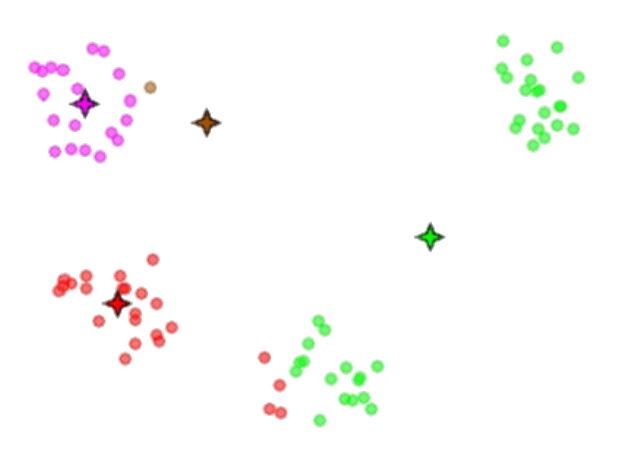
\includegraphics[height=180pt, keepaspectratio = true]{images/local_min4}  
\end{figure}
\end{frame}

\begin{frame}\frametitle{Чувствительность к начальному выбору $\mu_c$}
\begin{figure}[htbp]
  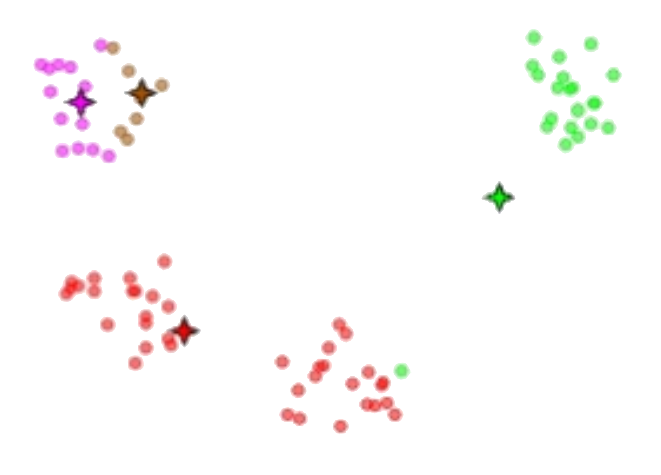
\includegraphics[height=180pt, keepaspectratio = true]{images/local_min6}  
\end{figure}
\end{frame}

\begin{frame}\frametitle{Чувствительность к начальному выбору $\mu_c$}
\begin{figure}[htbp]
  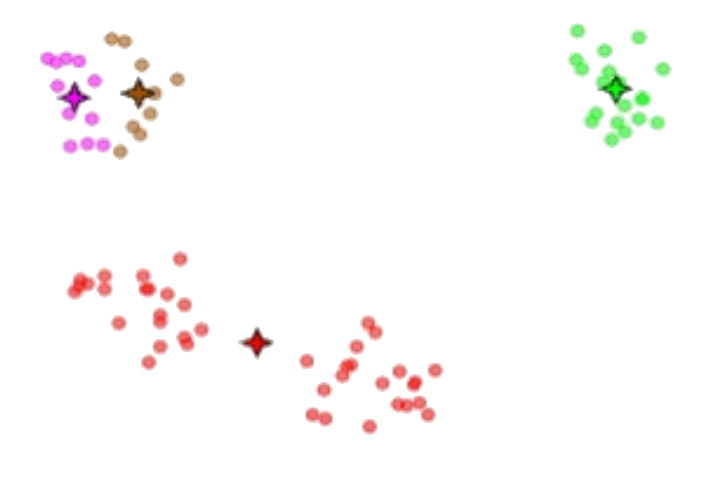
\includegraphics[height=180pt, keepaspectratio = true]{images/local_min7}  
\end{figure}
\end{frame}

\begin{frame}\frametitle{Необходимость задавать $k$}
\begin{figure}[htbp]
  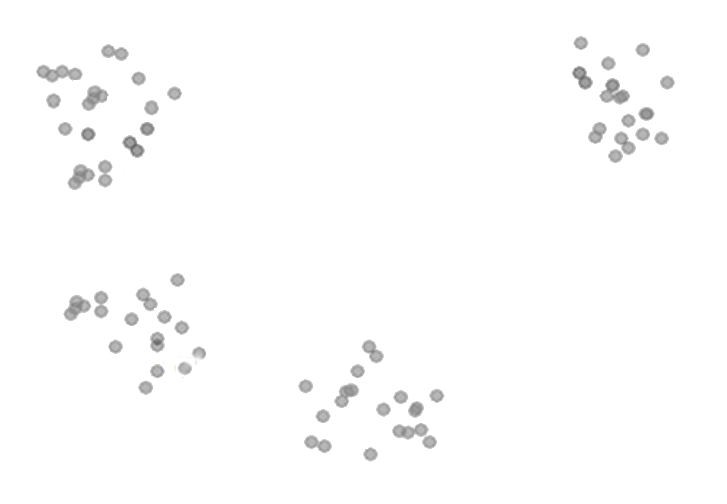
\includegraphics[height=180pt, keepaspectratio = true]{images/k_means_k}  
\end{figure}
\end{frame}

\begin{frame}\frametitle{Устранение недостатков}
\begin{itemize}
\item[--] Несколько случайных кластеризаций
\item[--] Постепенное наращивание числа $k$
\end{itemize}
\end{frame}

\begin{frame}\frametitle{Недостатки k-means}
\end{frame}

\begin{frame}\frametitle{"Не сферические данные"}
\begin{figure}[htbp]
  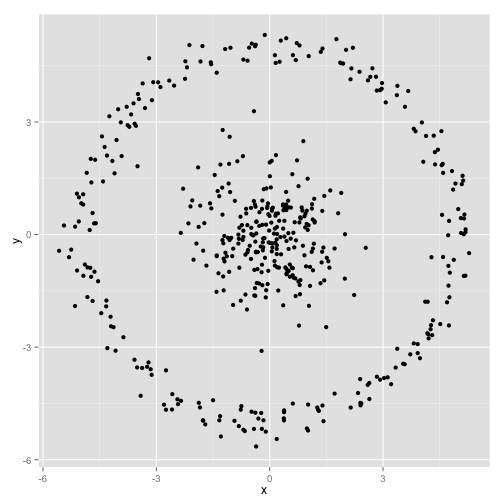
\includegraphics[height=180pt, keepaspectratio = true]{images/non_spherical-1}  
\end{figure}
\end{frame}

\begin{frame}\frametitle{"Не сферические данные"}
\begin{figure}[htbp]
  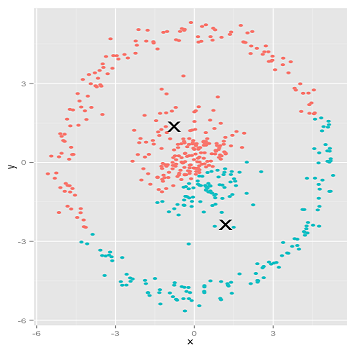
\includegraphics[height=180pt, keepaspectratio = true]{images/non_spherical-2}  
\end{figure}
\end{frame}

\begin{frame}\frametitle{"Не сферические данные"}
\begin{figure}[htbp]
  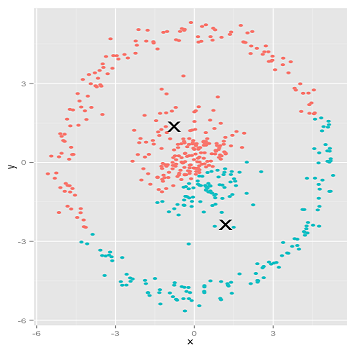
\includegraphics[height=180pt, keepaspectratio = true]{images/non_spherical-2}  
\end{figure}
\end{frame}

\begin{frame}\frametitle{Разноразмерные кластеры}
\begin{figure}[htbp]
  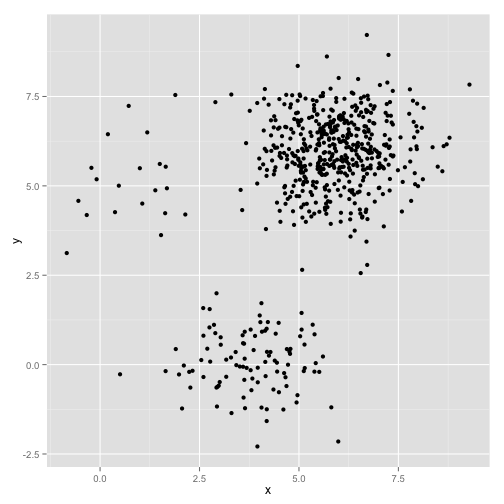
\includegraphics[height=180pt, keepaspectratio = true]{images/different_sizes-1}  
\end{figure}
\end{frame}

\begin{frame}\frametitle{Разноразмерные кластеры}
\begin{figure}[htbp]
  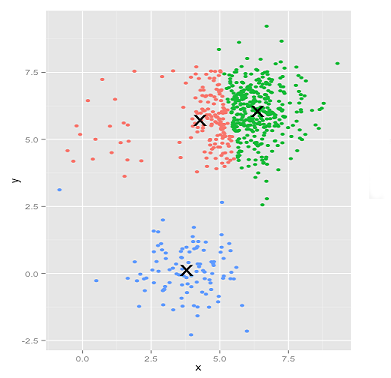
\includegraphics[height=180pt, keepaspectratio = true]{images/different_sizes-2}  
\end{figure}
\end{frame}

\begin{frame}\frametitle{На следующей лекции}
\begin{itemize}
\item[--] Линейные методы классификации
\item[--] Минимизация эмпирического риска
\item[--] Метод градиентного спуска
\item[--] Принцип максимума правдоподобия
\item[--] Балансировка ошибок и ROC-кривая
\end{itemize}
\end{frame}

\end{document}
